\documentclass[tikz]{standalone}

\usepackage{fontspec}

\usetikzlibrary{arrows}
\usetikzlibrary{calc}
\usetikzlibrary{decorations.pathreplacing}
\usetikzlibrary{positioning}
\usetikzlibrary{matrix}

\usepackage{fontspec}

\begin{document}

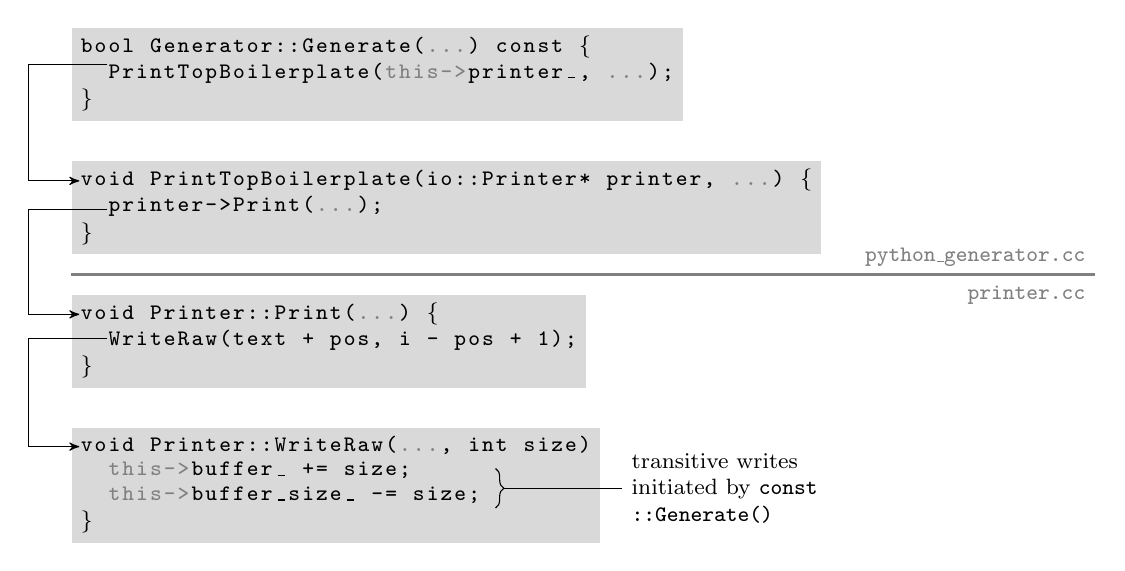
\begin{tikzpicture}
  [node distance=5mm, >=stealth',
  every node/.style={font=\footnotesize},
  every matrix/.style={fill=black!15, inner sep=1mm, row sep=0.5mm,
                        matrix of nodes, nodes in empty cells,
                        minimum height=0.5em, minimum width=.5em,
                        nodes={anchor=base, inner sep=0, font=\ttfamily\footnotesize}}]

  \matrix (Generate) {
b & o & o & l &   & G & e & n & e & r & a & t & o & r & : & : & G & e & n & e & r & a & t & e & ( & |[black!50]|. & |[black!50]|. & |[black!50]|. & ) &   & c & o & n & s & t &   & \{ &   &   &   &   &   &   \\
  &   & P & r & i & n & t & T & o & p & B & o & i & l & e & r & p & l & a & t & e & ( & |[black!50]|t & |[black!50]|h & |[black!50]|i & |[black!50]|s & |[black!50]|- & |[black!50]|> & p & r & i & n & t & e & r & \_ & , &   & |[black!50]|. & |[black!50]|. & |[black!50]|. & ) & ; \\
\} &   &   &   &   &   &   &   &   &   &   &   &   &   &   &   &   &   &   &   &   &   &   &   &   &   &   &   &   &   &   &   &   &   &   &   &   &   &   &   &   &   &   \\
  };

  \matrix [below=of Generate.south west, anchor=north west] (PrintTopBoilerplate) {
v & o & i & d &   & P & r & i & n & t & T & o & p & B & o & i & l & e & r & p & l & a & t & e & ( & i & o & : & : & P & r & i & n & t & e & r & * &   & p & r & i & n & t & e & r & , &   & |[black!50]|. & |[black!50]|. & |[black!50]|. & ) &   & \{ \\
  &   & p & r & i & n & t & e & r & - & > & P & r & i & n & t & ( & |[black!50]|. & |[black!50]|. & |[black!50]|. & ) & ; &   &   &   &   &   &   &   &   &   &   &   &   &   &   &   &   &   &   &   &   &   &   &   &   &   &   &   &   &   &   &   \\
\} &   &   &   &   &   &   &   &   &   &   &   &   &   &   &   &   &   &   &   &   &   &   &   &   &   &   &   &   &   &   &   &   &   &   &   &   &   &   &   &   &   &   &   &   &   &   &   &   &   &   &   &   \\
  };

  \matrix [below=of PrintTopBoilerplate.south west, anchor=north west] (Print) {
v & o & i & d &   & P & r & i & n & t & e & r & : & : & P & r & i & n & t & ( & |[black!50]|. & |[black!50]|. & |[black!50]|. & ) &   & \{ &   &   &   &   &   &   &   &   &   &   \\
  &   & W & r & i & t & e & R & a & w & ( & t & e & x & t &   & + &   & p & o & s & , &   & i &   & - &   & p & o & s &   & + &   & 1 & ) & ; \\
\} &   &   &   &   &   &   &   &   &   &   &   &   &   &   &   &   &   &   &   &   &   &   &   &   &   &   &   &   &   &   &   &   &   &   &   \\
  };

  \matrix [below=of Print.south west, anchor=north west] (WriteRaw) {
v & o & i & d &   & P & r & i & n & t & e & r & : & : & W & r & i & t & e & R & a & w & ( & |[black!50]|. & |[black!50]|. & |[black!50]|. & , &   & i & n & t &   & s & i & z & e & ) \\
  &   & |[black!50]|t & |[black!50]|h & |[black!50]|i & |[black!50]|s & |[black!50]|- & |[black!50]|> & b & u & f & f & e & r & \_ &   & + & = &   & s & i & z & e & ; &   &   &   &   &   &   &   &   &   &   &   &   &   \\
  &   & |[black!50]|t & |[black!50]|h & |[black!50]|i & |[black!50]|s & |[black!50]|- & |[black!50]|> & b & u & f & f & e & r & \_ & s & i & z & e & \_ &   & - & = &   & s & i & z & e & ; &   &   &   &   &   &   &   &   \\
\} &   &   &   &   &   &   &   &   &   &   &   &   &   &   &   &   &   &   &   &   &   &   &   &   &   &   &   &   &   &   &   &   &   &   &   &   \\
  };

  \draw[black!50, very thick] ($ (PrintTopBoilerplate.south west)!0.50!(Print.north west) $) -- ++(13cm, 0);
  \node [above, anchor=south east, black!50]
        at ($ (PrintTopBoilerplate.south west)!0.55!(Print.north west) + (13cm, 0) $)
        {\texttt{python\_generator.cc}};
  \node [below, anchor=north east, black!50]
        at ($ (PrintTopBoilerplate.south west)!0.55!(Print.north west) + (13cm, 0) $)
        {\texttt{printer.cc}};

  \draw [->] let \p1 = (Generate-2-3.north west),
                 \p2 = (PrintTopBoilerplate-1-1.west)
              in (\p1) -- ++(-1cm, 0) -- (\x1 - 1cm, \y2) -- (\p2);

  \draw [->] let \p1 = (PrintTopBoilerplate-2-3.west),
                 \p2 = (Print-1-1.west)
              in (\p1) -- ++(-1cm, 0) -- (\x1 - 1cm, \y2) -- (\p2);

  \draw [->] let \p1 = (Print-2-3.west),
                 \p2 = (WriteRaw-1-1.west)
              in (\p1) -- ++(-1cm, 0) -- (\x1 - 1cm, \y2) -- (\p2);


  \draw[decorate, decoration={brace, amplitude=3pt}]
       ($ (WriteRaw-2-30.north east) $)
       -- ($ (WriteRaw-3-30.south east)  $);
  \draw ($ (WriteRaw-2-30.north east)!0.5!(WriteRaw-3-30.south east) + (3pt, 0) $) -- ++(1.5cm, 0)
        node [right, text width=7em] {transitive~writes initiated~by {\tt \textbf{const}} {\tt ::Generate()}};

\end{tikzpicture}

\end{document}
